\chapter{Deep Networks for Equalization}

\section{Channel Estimation}

\begin{itemize}
\item compare least squares and how KNN did with pure deep nn based architecture
\item NN did better than least squares
\item hyperparam search over general 1-layer to 4-layer dense layers, and number of nodes and activations
\item plots: how error changed with respect to data points, as number of data points increased, NN outperformed LS
\item preamble: 100
\item want: QPSK, plot of preamble length
\item want? how to visualize that NN does better than LS
\end{itemize}




\section{Channel Equalization}

\subsection{Learning an inverse}

\begin{figure}
\begin{center}
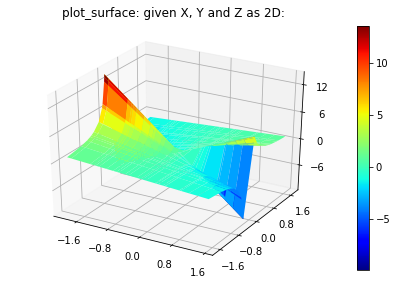
\includegraphics{figures/equal/Division_Function_plot.png}
\caption{Topographical surface representation of the division function; $z=\frac{x}{y}$.}
\end{center}
\label{fig:div_fx}
\end{figure}

\begin{figure}
\begin{center}
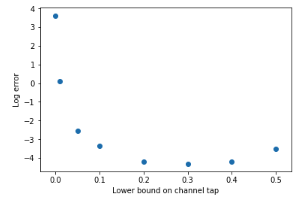
\includegraphics{figures/equal/One_tap_channel_inversion.png}
\caption{One tap channel inversion with respect to range.}
\end{center}
\label{fig:one_tap_inv}
\end{figure}

We explore whether a neural network can learn to do division.  

\begin{itemize}
\item can a NN learn to do division?
\item given a one tap channel and data sequence, output is equalized data sequence
\item with and without log feature scaling
\item without log errors = $10^-6$
\item MMSE gets error = $10^-32$
\item with log errors = 
\item straight inversion, without log feature scaling $10^-7$ - with dense layers
\item inversion with log feature scaling with error of $10^-14$ 
\item plots: inversion, but as a function of beta for both non-log and log
\end{itemize}


\subsection{Learning to multiply two inputs}
NN given x, y - output x*y

\begin{figure}
\begin{center}
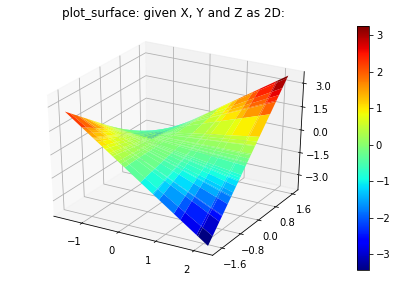
\includegraphics{figures/equal/Multiplication_Function_plot.png}
\caption{Topographical surface representation of the multiplication function; $z=xy$.}
\end{center}
\label{fig:mult_fx}
\end{figure}

\begin{figure}
\begin{center}
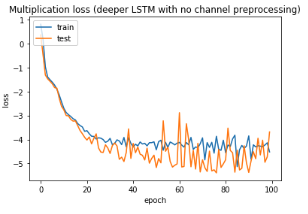
\includegraphics{figures/equal/LSTM_loss_multiplication.png}
\caption{LSTM loss trying to learn the Multiplication function; $z=xy$.}
\end{center}
\label{fig:lstm_loss_mult}
\end{figure}

\begin{figure}
\begin{center}
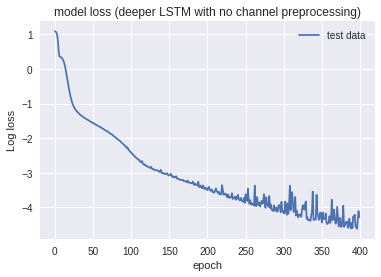
\includegraphics{figures/equal/Multiplication_loss_vs_epoch.png}
\caption{LSTM loss trying to learn the Multiplication function; $z=xy$.}
\end{center}
\label{fig:loss_mult}
\end{figure}

\begin{figure}
\begin{center}
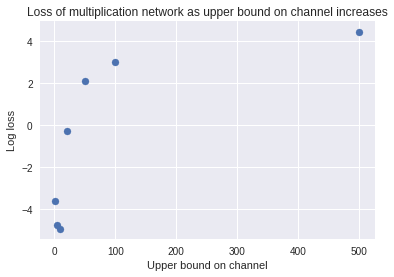
\includegraphics{figures/equal/Channel_upper_bound_multiplication.png}
\caption{LSTM loss trying to learn the Multiplication function; $z=xy$.}
\end{center}
\label{fig:mult_bound}
\end{figure}

\subsection{RNN for Channel Equalization}

\begin{itemize}
\item compare to MMSE
\item re run with the new RNN architecture
\item backprop length of ~ 3. crude search from 1-10. 2 tap channel
\item added channel preprocessing: didn't seem to make too much of a difference
\item plot log/ log scale to find converging in error
\end{itemize}

\begin{figure}
\begin{center}
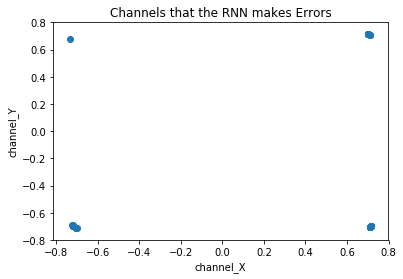
\includegraphics[width=100mm]{figures/equal/incorrect_channels.png}
\caption{What two tap channels does the equalizer get wrong?}
\label{fig:incorr_chan}
\end{center}
\end{figure}

Figure~\ref{fig:incorr_chan} shows which channels the RNN equalizer and classic demodulator got any bits wrong.  
There were a total of $50k$ random channels in the test set.  
Of that set, only $43$ channels resulted in incorrect bits after the RNN equalizer and classic demodulator.
From the figure, it is clear that these difficult channels are clustered into four regions. All of the four regions are when the first and second tap of the channel are equal in magnitude.
The mean squared error between the equalized data and the true data among just the bad channels was $0.7306$.  The mean squared error among the good channels was $0.000264$.

\begin{align*}
\begin{bmatrix}
\text{Tap 1} & \text{Tap 2} & \text{Counts of bad estimates} & \text{Mean Squared Error}\\
\hline
0.707 & 0.707 & 14 & 0.7162\\
-0.707 & 0.707 & 1 & 0.5236\\
0.707 & -0.707 & 16 & 0.8172\\
-0.707 & -0.707 & 12 & 0.6492\\
\end{bmatrix}
\end{align*}


